

\begin{figure}[H]
	\centering
	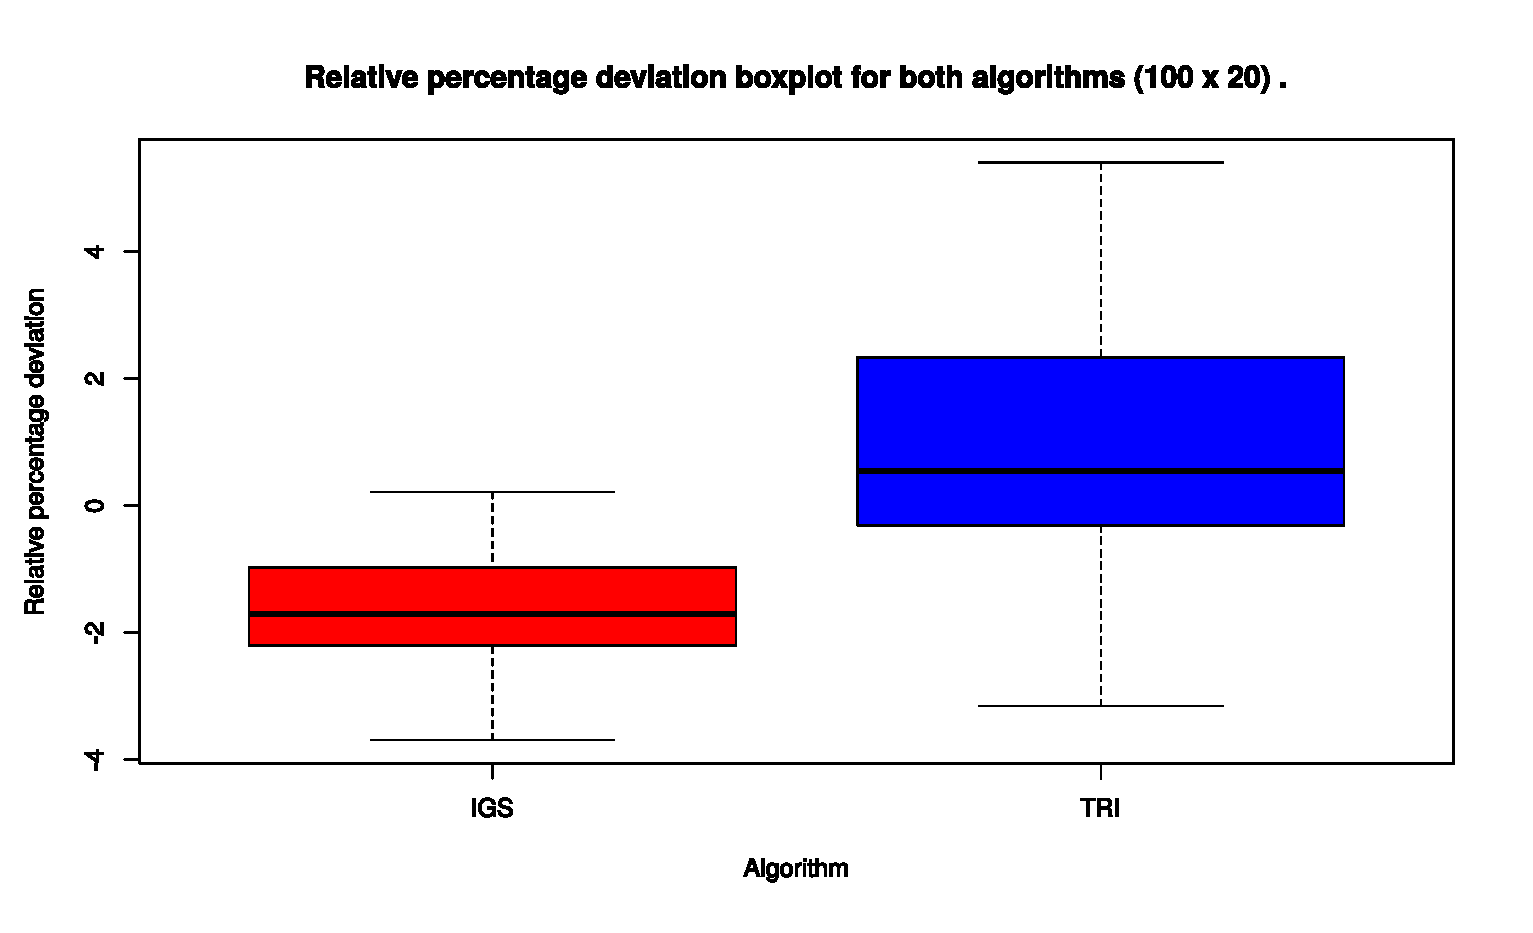
\includegraphics[width=\textwidth]{fig/box/100x20}
	\caption{Relative percentage deviation boxplot ($100 \times 20$)}
\end{figure}

\begin{figure}[H]
	\centering
	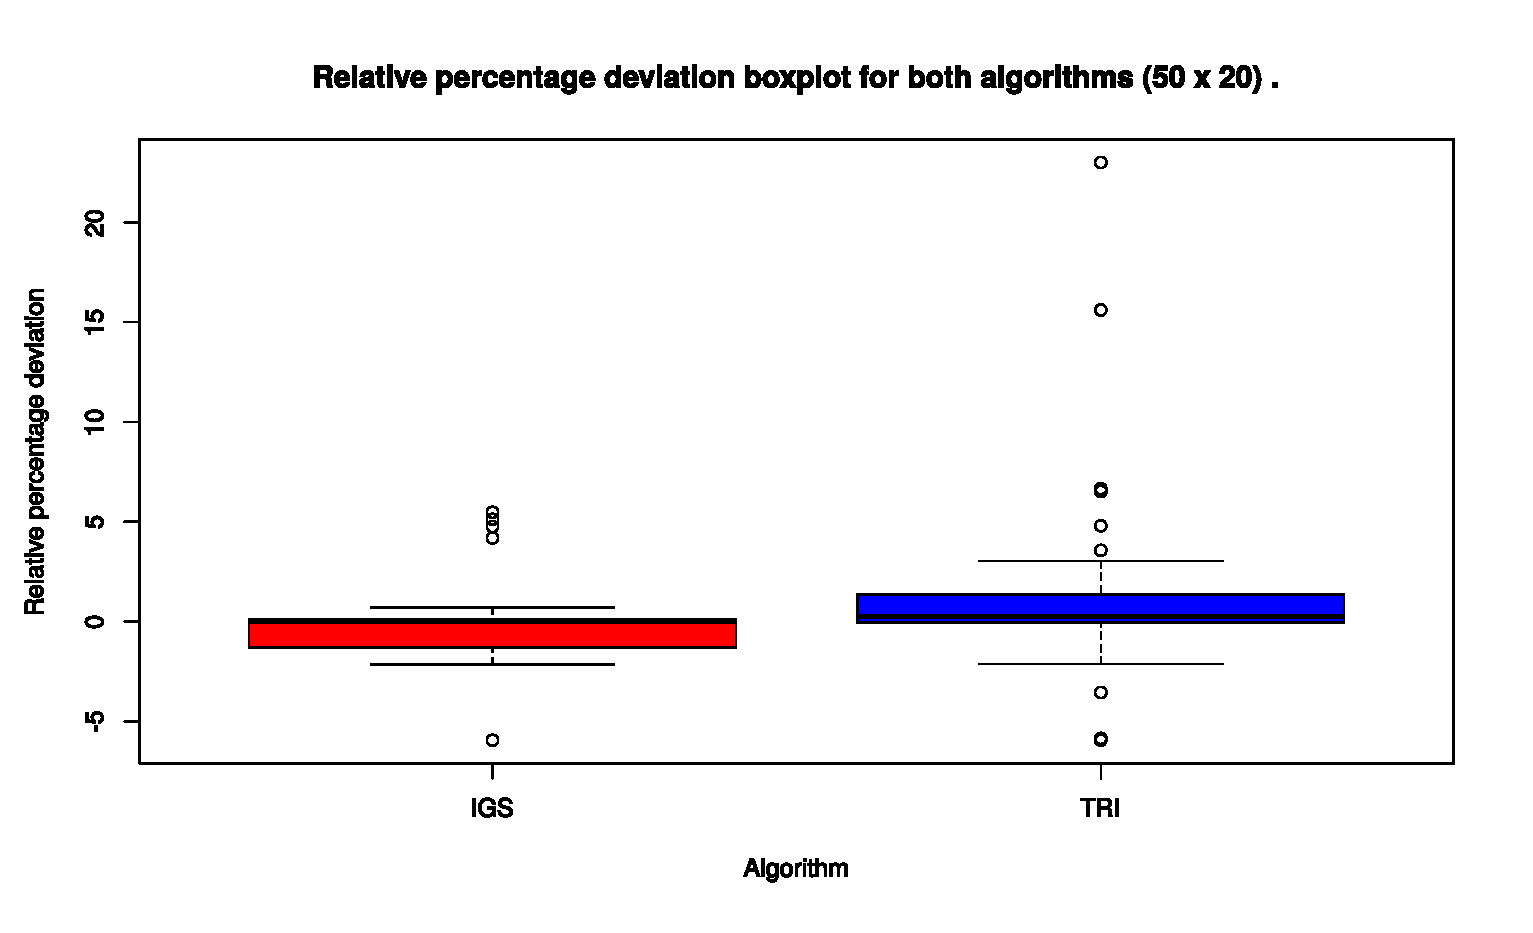
\includegraphics[width=\textwidth]{fig/box/50x20}
	\caption{Relative percentage deviation boxplot ($50 \times 20$)}
\end{figure}

\begin{figure}[H]
	\centering
	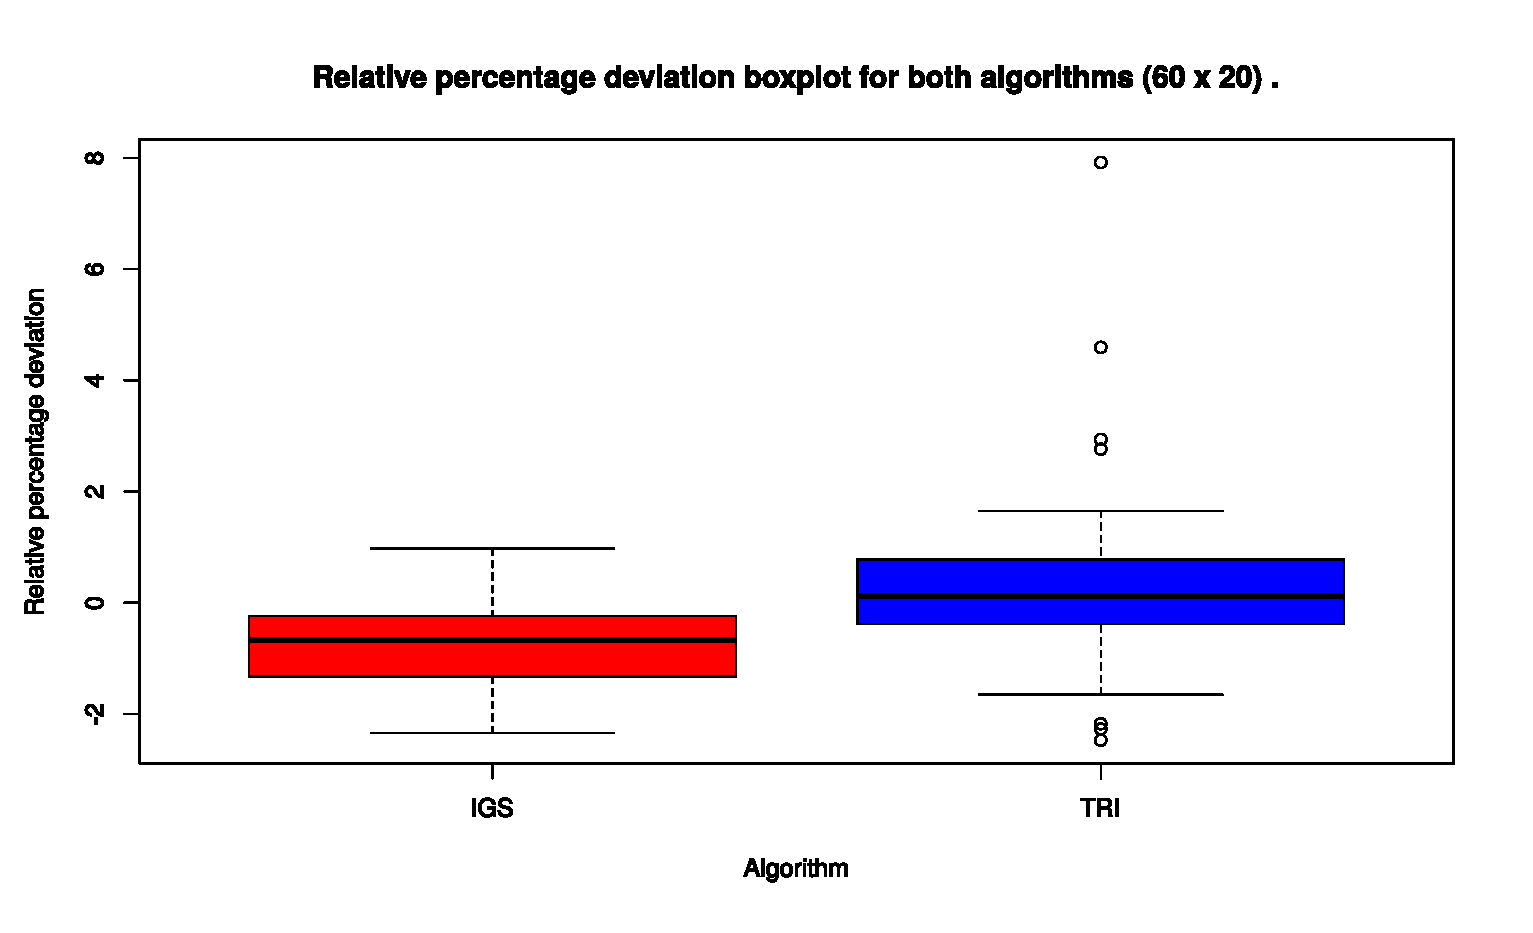
\includegraphics[width=\textwidth]{fig/box/60x20}
	\caption{Relative percentage deviation boxplot ($60 \times 20$)}
\end{figure}

\begin{figure}[H]
	\centering
	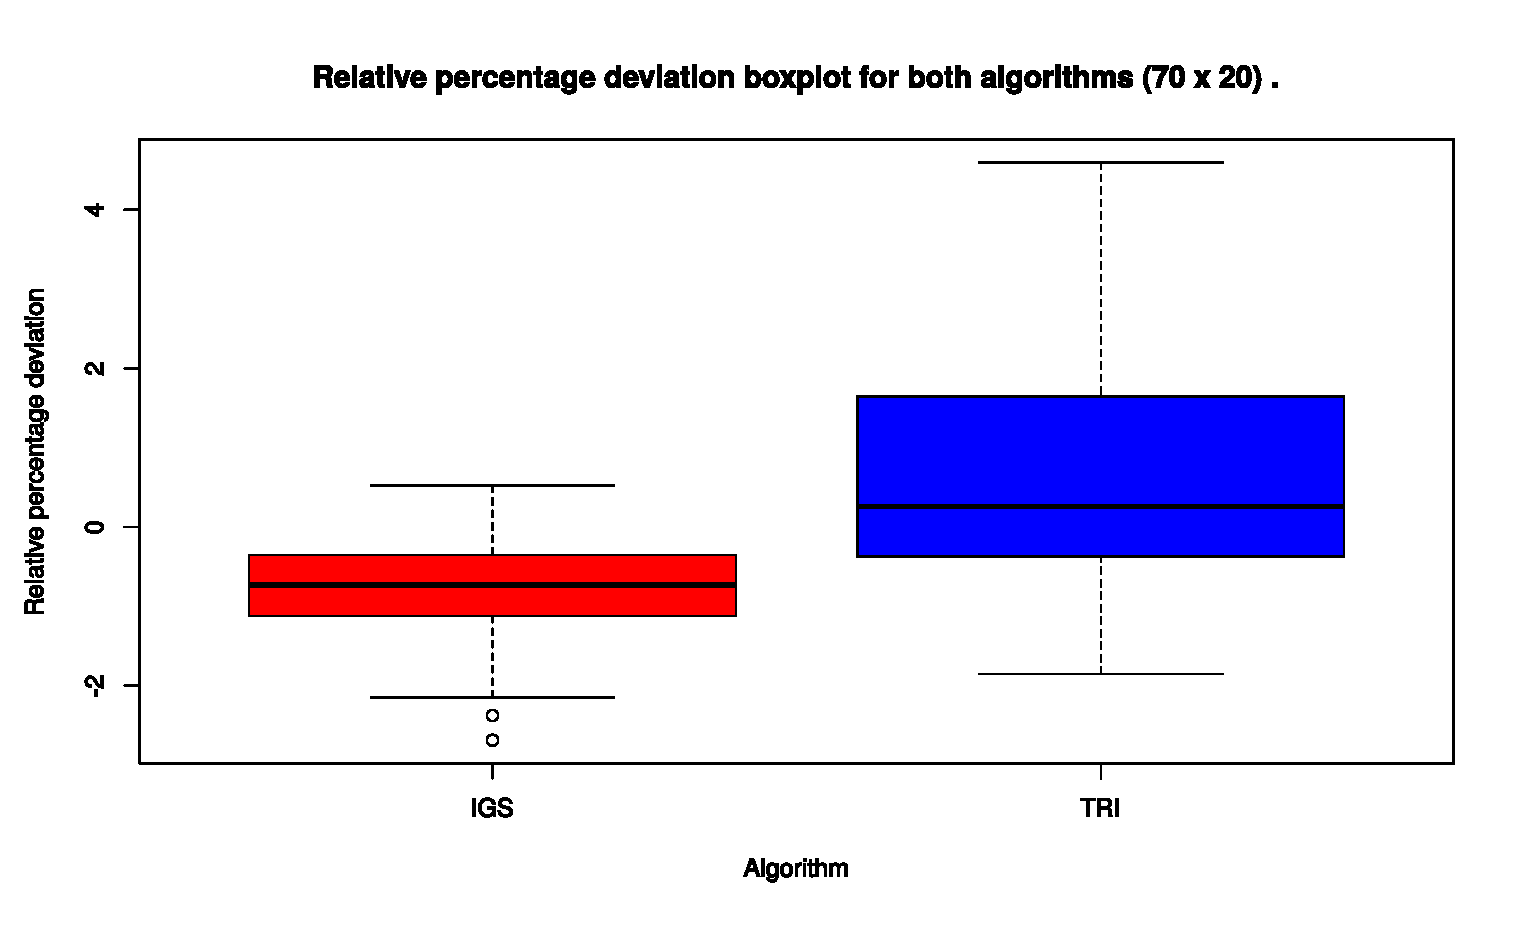
\includegraphics[width=\textwidth]{fig/box/70x20}
	\caption{Relative percentage deviation boxplot ($70 \times 20$)}
\end{figure}

\begin{figure}[H]
	\centering
	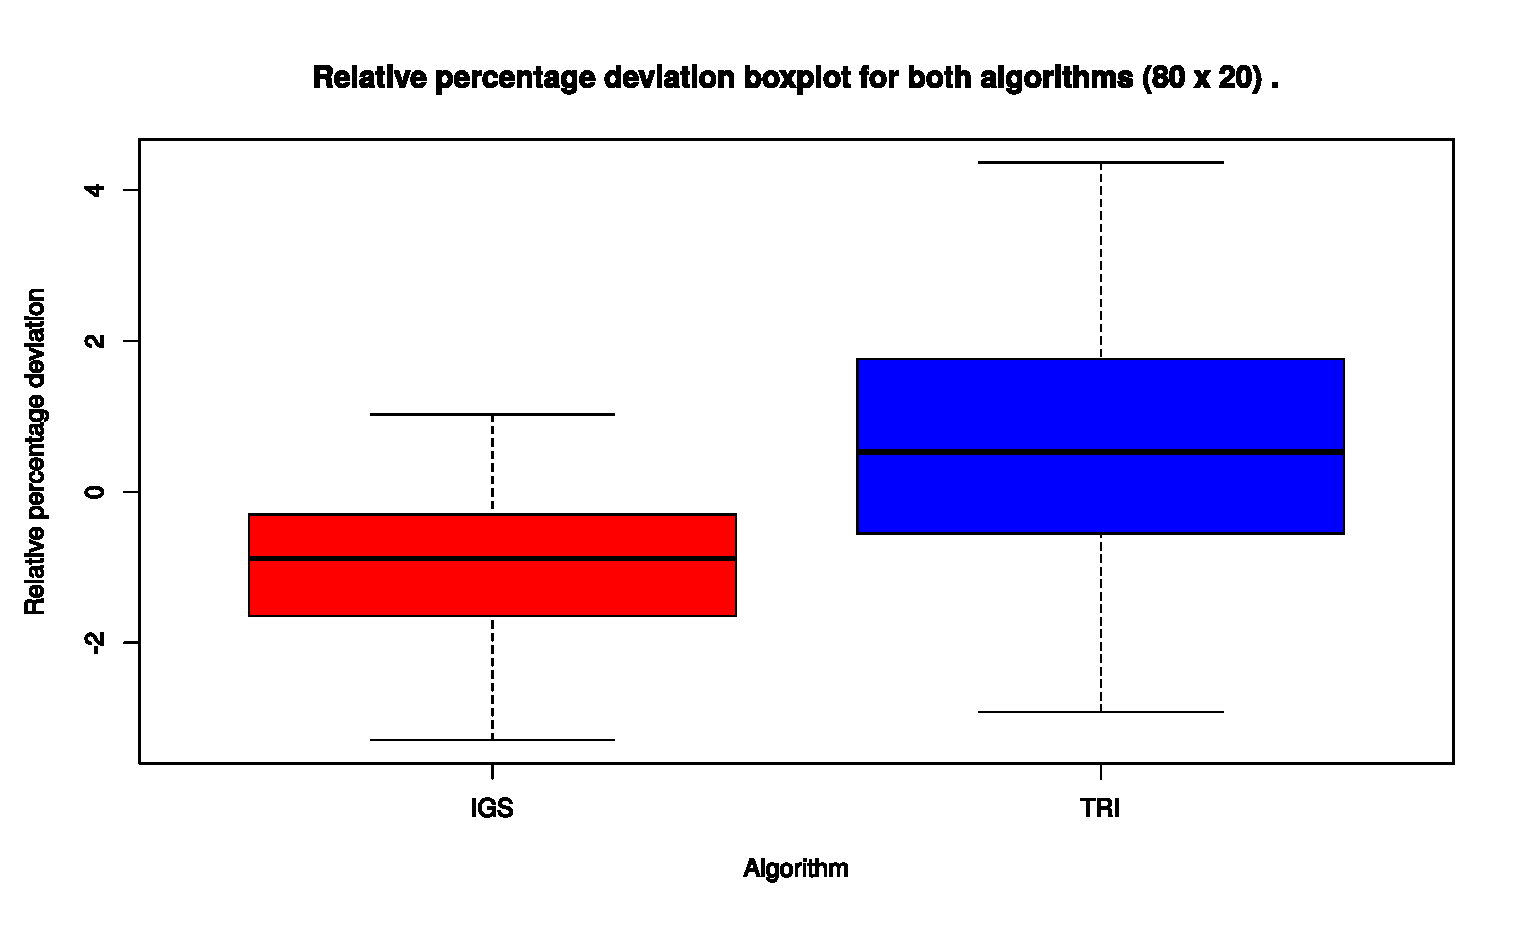
\includegraphics[width=\textwidth]{fig/box/80x20}
	\caption{Relative percentage deviation boxplot ($80 \times 20$)}
\end{figure}

\begin{figure}[H]
	\centering
	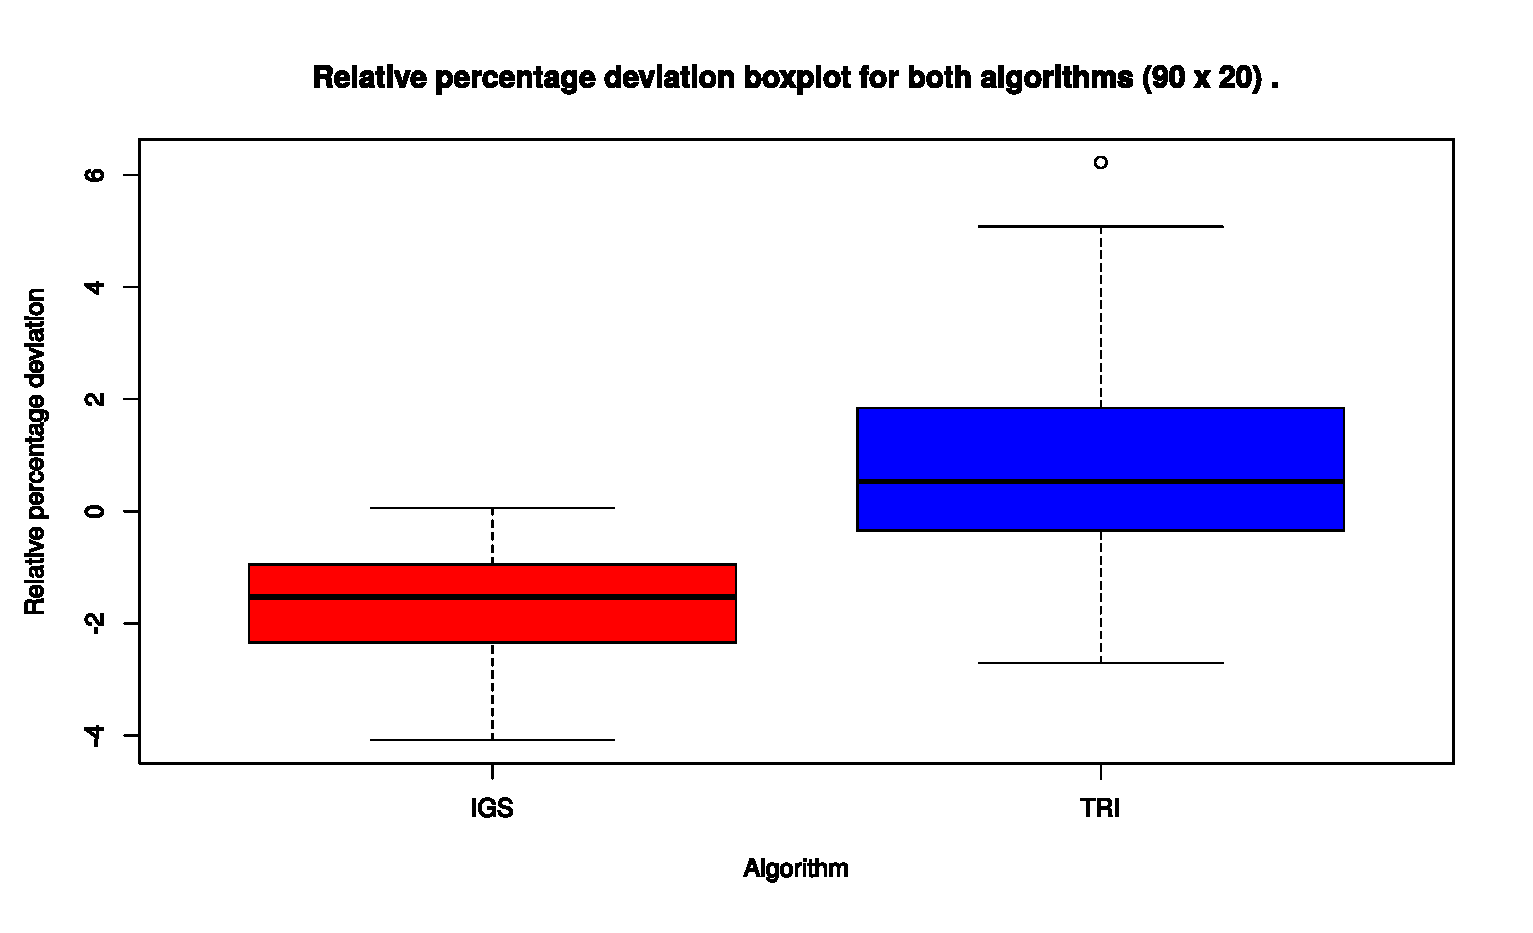
\includegraphics[width=\textwidth]{fig/box/90x20}
	\caption{Relative percentage deviation boxplot ($90 \times 20$)}
\end{figure}